\chapter{Introduction}

%%%%%%%%%%%%%%%%%%%%%%%%%%%%%%%%%%%%%%%%%%%%%%%%%%%%%%%%%%%%%%%%%%%%%%%%%%%%%%%%
%%  Motivation (aus MDE4BPM'08-Paper)                                         %%
%%%%%%%%%%%%%%%%%%%%%%%%%%%%%%%%%%%%%%%%%%%%%%%%%%%%%%%%%%%%%%%%%%%%%%%%%%%%%%%%

The goal of process modeling, as of Model Driven Engineering in general, is to
provide an abstract view on systems, and to design those systems in a language
and platform independent way.  For that purpose the Business Process Modelling
Notation (BPMN)~\cite{omg2009bpmn} standard was created by the Object Management
Group.  It can be understood intuitively by all business partners, even those who
have great knowledge in their domain but do not know too much about Service
Oriented Architecture (SOA) or programming in general.  At the same time, BPMN is
formal enough to provide a basis for the later implementation and refinement of
the business process.  Given a respective mapping, a BPMN diagram can be used for
generating readily executable code from it.  A brief introduction to BPMN is given
for instance in~\cite{white2004introduction} and in Appendix~\ref{sec:bpmn} of
this manual.

Today, the Business Process Modelling Notation and the specified mapping to the
Business Process Execution Language (BPEL) are supported by a growing number of
tools.  However, the problem with the majority of existing tools is that while
they do provide the usual transformations from BPMN to BPEL, they are focused
only on this one aspect of BPMN.  Often the editors and even the underlying
meta-models are adapted to BPEL in many ways.  While this may be desired in order
to provide highest possible usability and to support the user in the creation of
executable BPEL code, the consequence is that business process diagrams created
with these tools can neither be transformed to other executable languages, nor
can the process model be used with other tools that might provide different
transformations.  Thus, while process modeling and BPMN should be independent of
a specific executable language, the \emph{tools} are not.

The solution to this problem is to keep both the underlying BPMN meta-model and
the diagram editor free from influences from the BPEL world and to use pure BPMN
instead, so that diagrams created with such a tool will be truly independent of
any concrete language -- apart from what influenced the BPMN specification in
the first place.  Based on this, several mappings to different target languages
can be implemented and integrated into the editor as plug-ins, which may also
contribute to the editor in order to support the business architect with
language-specific support.

Following this approach, the \emph{Visual Service Design Tool} (VSDT) has been
implemented as an Eclipse plug-in, inherently providing the necessary modularity.
For the export of BPMN diagrams to executable languages a transformation framework
has been designed.  The actual transformations have been subdivided in distinct
stages, so that significant parts of it are reusable, e.g.\ the challenging
transformation of the control flow.  Thus the actual mapping to a given language
can be integrated in a very straight-forward way.  While the usual mapping from
BPMN to BPEL has been realized as a proof of concept, the main intent behind the
VSDT is to provide a transformation from business processes to multi-agent systems
such as the JIAC language family~\cite{hirsch2009jiacv}.  The respective mappings
are currently under development.  Our ultimate goal is to provide transformations
not only in different, but also in heterogeneous systems just like they are used
in the real business world.


%%%%%%%%%%%%%%%%%%%%%%%%%%%%%%%%%%%%%%%%%%%%%%%%%%%%%%%%%%%%%%%%%%%%%%%%%%%%%%%%
%%  Features                                                                  %%
%%%%%%%%%%%%%%%%%%%%%%%%%%%%%%%%%%%%%%%%%%%%%%%%%%%%%%%%%%%%%%%%%%%%%%%%%%%%%%%%

\section{The Visual Service Design Tool}

The first version of the VSDT has been developed as a diploma
thesis~\cite{kuester2007dipl} in the course of the \emph{Service Centric Home
(SerCHo)} project at TU Berlin in early 2007.  As the work continued, it matured
to a feature-rich BPMN editor (as seen in Figure~\ref{fig:screen}) with an
extensible transformation framework and has already been used in a number of
service orchestration scenarios.

\begin{figure}
	\centering
	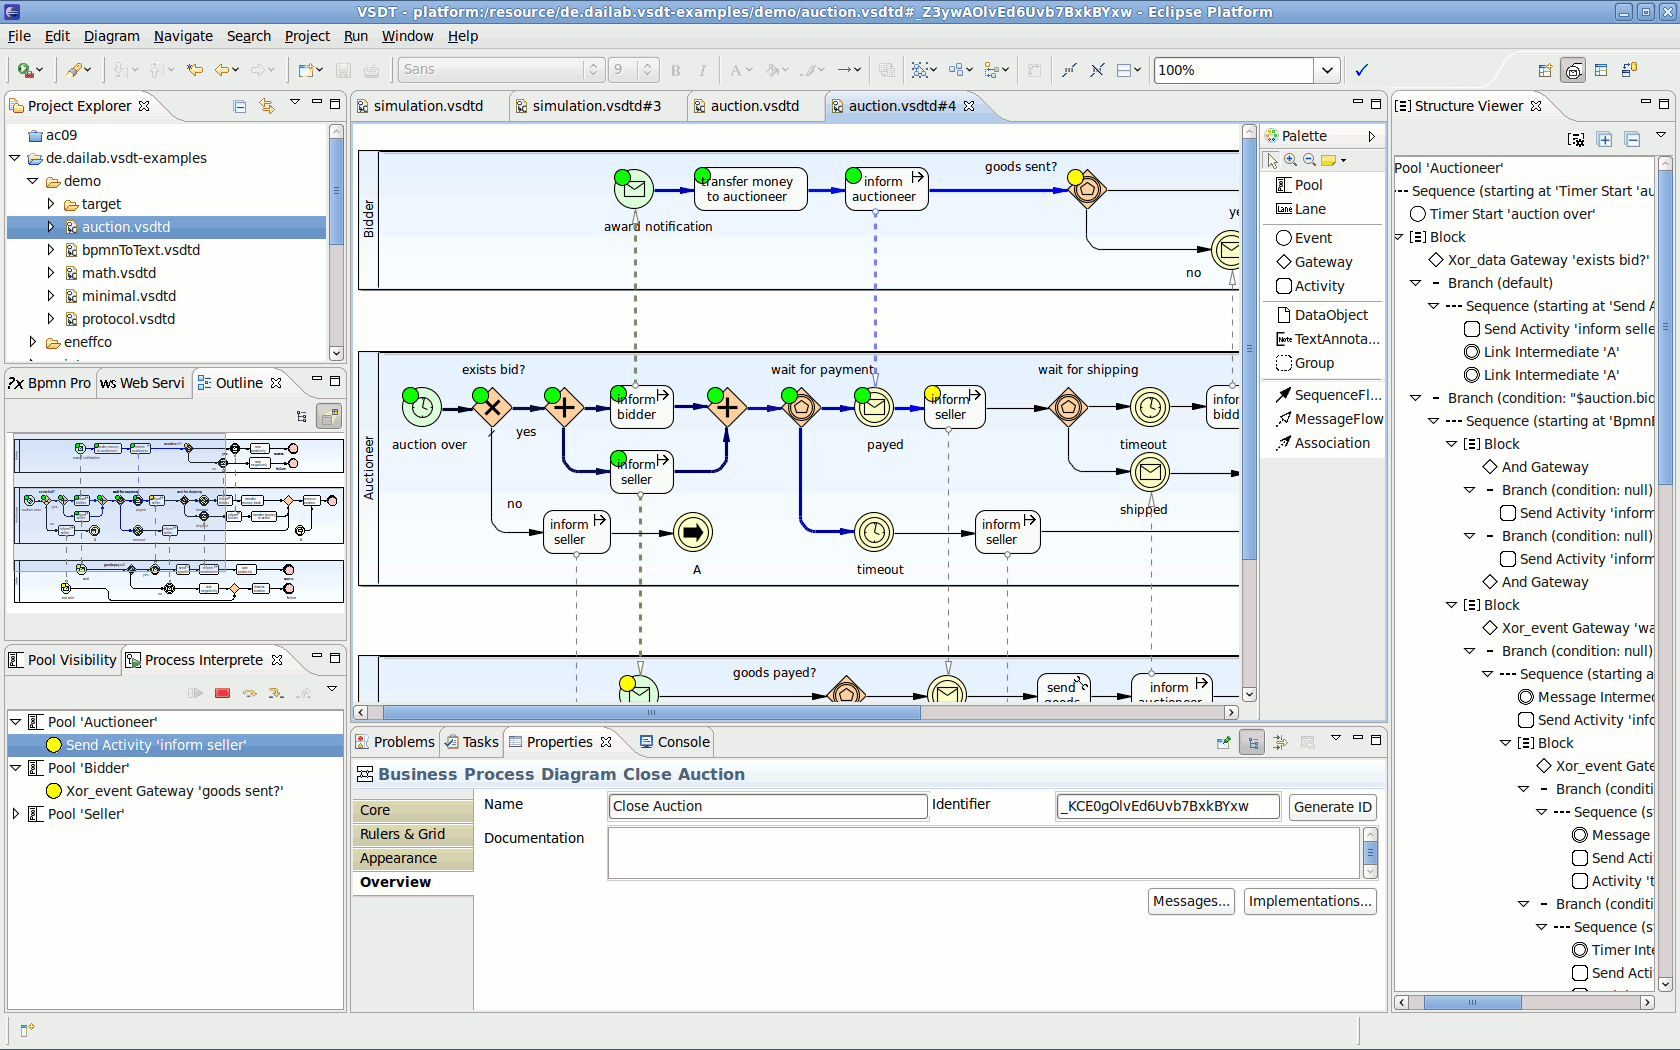
\includegraphics[height=.4\textheight]{figures/vsdt_1-3-0.png}
	\caption[The Visual Service Design Tool]{The Visual Service Design Tool.
	Clockwise: Graphical Editor (with running Simulation), Structure Viewer,
	Property View, Process Interpreter View, Visual Outline, Navigator.}
	\label{fig:screen}
\end{figure}


\subsection{The Metamodel}

% Ueber die BPMN Spezifikation und wie sie umgesetzt wurde
The BPMN specification~\cite{omg2009bpmn} describes in detail how the several
nodes and connections constituting a BPMN diagram have to look, in which context
they may be used and what attributes they have to provide.  However, it does
neither give a formal definition of the syntax to be used for the meta-model, nor
an interchange format, e.g. using an XML Schema Definition (XSD).  Thus the
editor's meta-model had to be derived from the informal descriptions in the
specification.  As it was our main concern to keep as close to the specification
as possible, almost every attribute and each constraint given in the specification
have been incorporated into the meta-model, allowing the creation of any legal
business process diagram.  Still, some attributes have not been adopted in the
meta-model: For instance the possibility to model nested or even crossing Lanes
has been dropped, as it turned out that this feature seems to be virtually never
used in practical business process design.


\subsection{The BPMN Editor}

% Basis: Eclipse GMF -> Viele gute Features frei Haus
Like many others, the VSDT editor has been created using the \emph{Eclipse Graphical
Modelling Framework (GMF)}, automatically equipping the editor with numerous
features, such as support for the Eclipse properties, outline and problem view
and unlimited undo and redo, just to name a few.  Being embedded in the Eclipse
workbench, the editor is easy to use while at the same time providing a powerful
tool for professional business architects and service developers.

% Erweiterungen: Property Sheets, Dialoge, Validierung, etc.
While GMF provides a solid basis for the editor, several customizations have been
made to the code, further improving the editor's overall usability and supporting
the creation of new business processes.  For example, the generated property
tables have been supplemented with custom-made sheets, in which the several
attributes are more clearly arranged.  For managing the non-visual elements given
in the BPMN specification, such as Properties, Messages and Assignments, a number
of clear and uniform dialogs were created.  The various constraints given in the
specification were translated to several audit constraints used to validate a
given business process diagram.

% Nachteil der Erweiterbarkeit/ BPEL-unabhaengigkeit: keine BPEL-Untertuetzung im Editor
As already mentioned, the VSDT was designed to be a pure BPMN editor and independent
of BPEL, so the business process diagrams can be transformed to other languages,
too, given the respective export plug-ins.  Of course, the downside of this approach
is that the editor lacks built-in support for BPEL, e.g.\ the editor itself does
not validate an expression given in the diagram to conform to the BPEL syntax.
However, it is possible to supplement the editor with additional plug-ins, which
can contribute e.g.\ to the property sheets or provide whole new views with
language-specific functionality.

% Rich Service Directory
One example of how the VSDT can be extended with features specific to a certain
target language -- in this case: BPEL -- is the Web Service View, which can bee
seen in Figure~\ref{fig:screen}, too.  Using the Web Service View, existing Web
services can be inspected and imported into the diagram.  In the process, an
Implementation object is created for the Web service as well as a set of Message
objects, matching the service's input parameters and result.  Optionally, also a
new Pool will be created for the service, which can be connected to the currently
selected Activity via a pair of Message Flows.  Further, the Implementation and
the Message objects will be associated to the Activity and its type will be set
to \textsc{service}.  Thus, the orchestration of existing Web services in a BPEL
process can be simplified greatly.  Similar features can be created for other
target languages, too.

% Export Wizards
Once the business process diagram is completed, it can be validated and exported
to an executable language, such as BPEL or the JIAC agent framework.  As the VSDT
is intended to provide export features to arbitrary target languages, and to
support developers in the creation of these features, we have created an elaborate
export framework.  For each of these features, being realized as additional
Eclipse plug-ins, an individual wizard can be made available in the Export menu.

For more information regarding the Visual Service Design Tool, please refer
to~\cite{kuester2008vsdt}.


%%%%%%%%%%%%%%%%%%%%%%%%%%%%%%%%%%%%%%%%%%%%%%%%%%%%%%%%%%%%%%%%%%%%%%%%%%%%%%%%
%%  Features                                                                  %%
%%%%%%%%%%%%%%%%%%%%%%%%%%%%%%%%%%%%%%%%%%%%%%%%%%%%%%%%%%%%%%%%%%%%%%%%%%%%%%%%

\section{Features}

% Stand: Version 1.4.0

In the following, some of the features of the VSDT are listed.  For more information
on selected features, please refer to Section~\ref{sec:user_features}.

\begin{itemize}
	\item export to executable BPEL and JIAC Code% and STP-BPMN
	\item translation of Expressions to the language used in the target framework
	\item process simulation and interpretation
	\item BPMN-to-text generation
	\item combination of BPMN-diagrams with Use-case-like 'higher view'
	\item pattern-based modeling, insertion of pattens on existing edges
	\item quick assembly of process diagrams using keyboard-shortcuts
	\item quick assignment of service parameters
	\item dynamic filtering of displayed pools
	\item variables-view and similar tools for the management of non-visual elements
	\item verification of process structure at design time
	\item automated, structure-based layout of BPMN diagrams
	\item one-click deployment of JIAC agent services generated from BPMN diagrams on a JIAC runtime
\end{itemize}

